\section{Evaluation}

To demonstrate the performance and correctness of our ZOne implementation, we
present three benchmark: convolution, BlackScholes, and histogram.
While all three befinit greatly from our I/O latency interleaving, we show
	that histogram also improves from our compiler optimizations.


\subsection{Vector Add}

\subsection{Convolution}
Convolutions have many uses in engineering and mathematics, particularly in
the image-processing fields. High-performance CPU convolution imlpementations
involve vectorization and tiling to make full use of cache bandwidth and 
execution resources. The ZOne convolution code is figure~\ref{fig:stencil}.

\begin{figure}
\centering
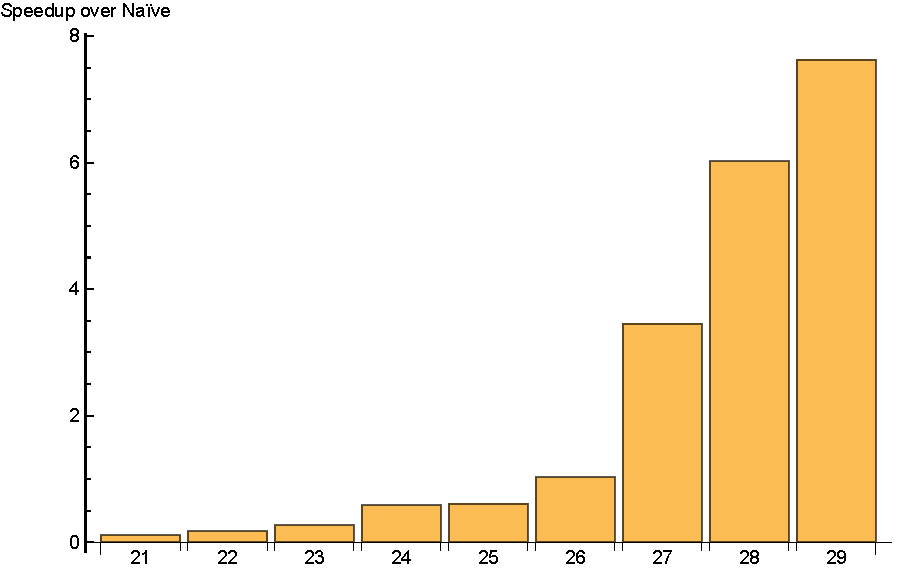
\includegraphics[scale=0.5]{data/stencil.pdf}
\caption{Speedup over CUDA verion..todo}
\label{fig:stencil}
\centering
\end{figure}


\subsection{Histogram}
Histograms are a fundamental analysis tool in image and data processing.
Efficient serial CPU histogram implementations are very straghtforward, but
due to the data-dependant access pattern efficient GPU implementations are
more involved. They typically feature privitization,
where individual histograms for portions of the data are computed separately
and then compiled together into the overall result. This reduces serialization
of atomic memory accesses when different threads increment the same bin.
Other approaches include sorting the input data and then finding the start
index of each bucket, and approaches that use graphics-specific hardware like
occlusion queries.

\begin{figure}
\centering
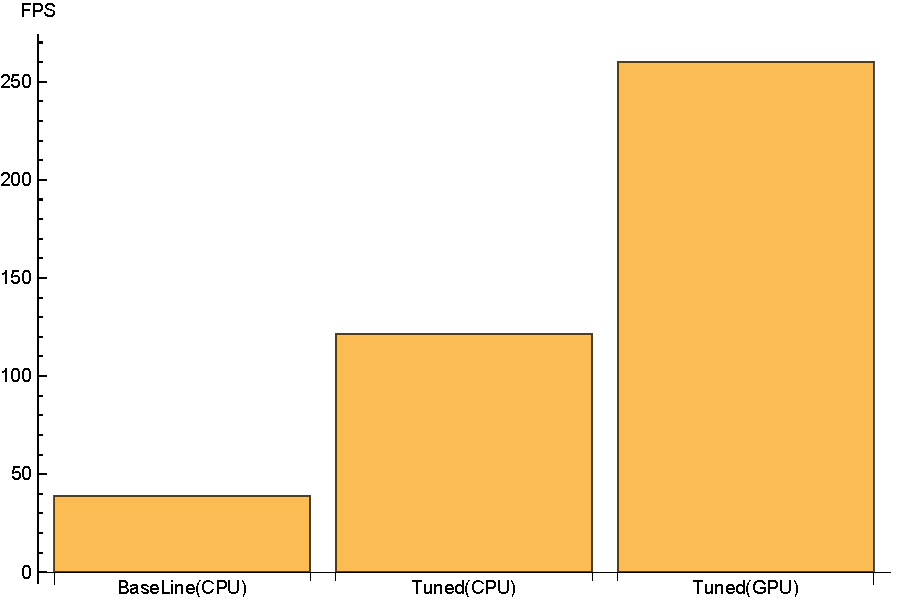
\includegraphics[scale=0.5]{data/histogram.pdf}
\caption{Frames per seconds achieved for histogram equalization kernel on a 4K video. The figure compares the tuned GPU implementation to a naive CPU and tuned CPU implementations. The tuned GPU implementation uses thread coarsining to achieve high fps.}
\label{fig:histogram}
\centering
\end{figure}


\begin{figure}
\centering
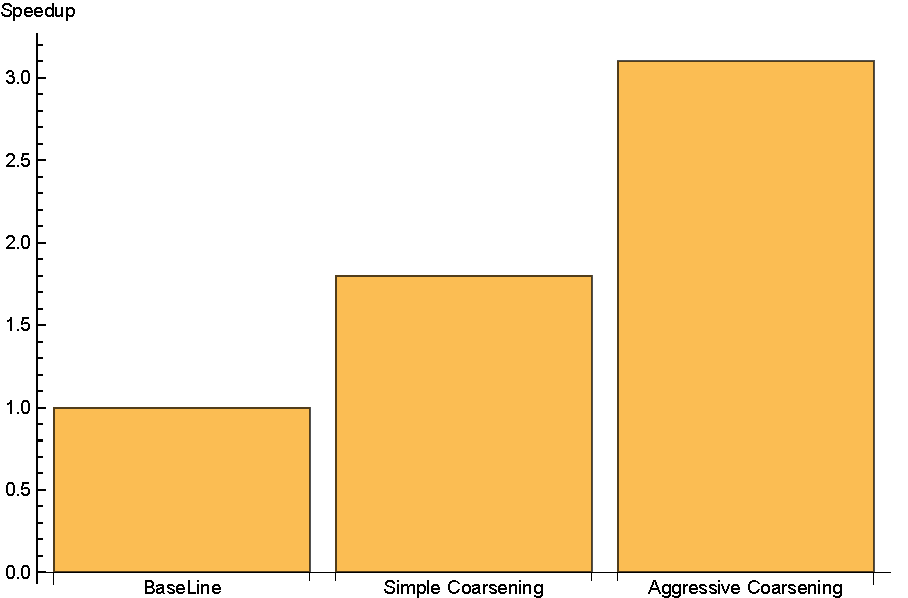
\includegraphics[scale=0.5]{data/histogramc.pdf}
\caption{The coarsining parameter impacts the performance of the histogram equalization kernel.}
\label{fig:histogramCoarsining}
\centering
\end{figure}

\subsection{Black-Scholes}
Black-Scholes models option pricing by simplifying ito's formula, and some other stuf....



\begin{figure}
\centering
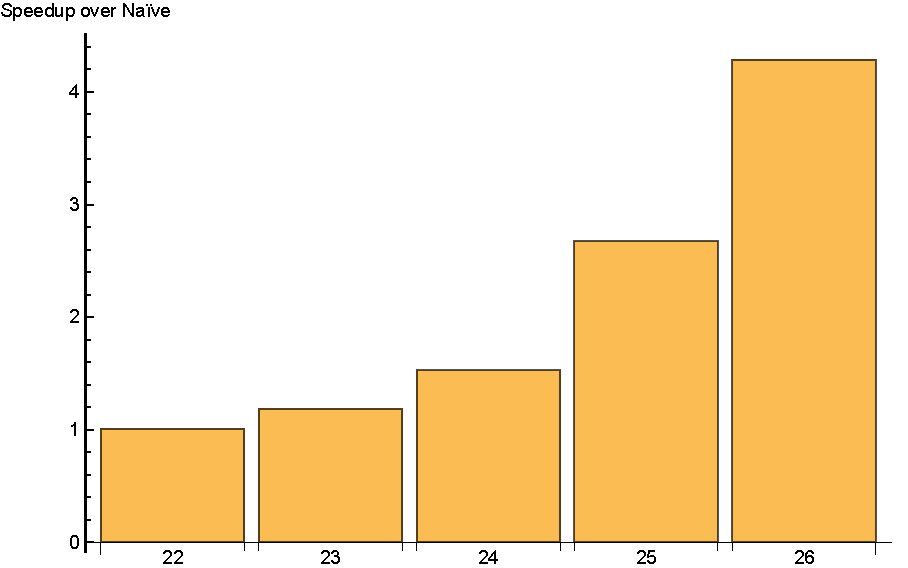
\includegraphics[scale=0.5]{data/blackscholes.pdf}
\caption{Speedup over CUDA verion..todo}
\label{fig:blackscholes}
\centering
\end{figure}


\subsection{European Pricing}

